\chapter{Bosones compuestos, representaciones de espín y duplicación de Dirac}

\section{Simetría de intercambio y bosones compuestos}

La pregunta inicial plantea una paradoja genuina sobre las partículas compuestas. Si dos fermiones forman un bosón, ¿pueden dos de esos bosones ocupar el mismo estado sin violar la exclusión fermiónica? La respuesta parte de la propia regla de intercambio.

Supongamos que una función de onda de dos argumentos describe dos partículas idénticas. Los símbolos \(x\) y \(y\) designan los dos lugares correspondientes a las partículas; no distinguen dos especies. Para los bosones, la función de onda es simétrica; para los fermiones, es antisimétrica:
\begin{equation}
\Psi_B(x,y)=\Psi_B(y,x),
\qquad
\Psi_F(x,y)=-\Psi_F(y,x).
\end{equation}
La simetría expresa que intercambiar las dos partículas indistinguibles no produce un nuevo estado físico.

Es perfectamente posible que dos bosones ocupen el mismo estado de una partícula. Si ese estado tiene la función de onda \(\varphi\), el producto para dos partículas es
\begin{equation}
\Psi(x,y)=\varphi(x)\varphi(y).
\end{equation}
Las funciones de onda son funciones ordinarias con valores complejos, no operadores ni matrices, por lo que sus valores conmutan:
\begin{equation}
\varphi(x)\varphi(y)=\varphi(y)\varphi(x).
\end{equation}
Por tanto, el producto es simétrico. La misma construcción no puede producir un estado no nulo de dos fermiones, pues la antisimetría exigiría
\begin{equation}
\varphi(x)\varphi(y)=-\varphi(y)\varphi(x),
\end{equation}
aunque los dos lados sin el signo menos son iguales.

Más en general, partamos de cualquier función de onda de dos partículas \(F(x,y)\), sin suponer que tenga simetría de intercambio. Sus partes simétrica y antisimétrica son, salvo un factor de normalización,
\begin{align}
F_{\mathrm{sym}}(x,y)&=F(x,y)+F(y,x),\\
F_{\mathrm{asym}}(x,y)&=F(x,y)-F(y,x).
\end{align}
La comprobación del intercambio es explícita:
\begin{align}
F_{\mathrm{sym}}(y,x)
&=F(y,x)+F(x,y)
=F_{\mathrm{sym}}(x,y),\\
F_{\mathrm{asym}}(y,x)
&=F(y,x)-F(x,y)
=-F_{\mathrm{asym}}(x,y).
\end{align}
Sumar la función intercambiada la simetriza; restarla la antisimetriza.

Un par de átomos de hidrógeno ofrece un caso más interesante. Hay cuatro fermiones constituyentes: dos electrones idénticos y dos protones idénticos. Sea \(x_1,x_2\) el conjunto de variables de los electrones y \(y_1,y_2\) el de los protones. La función de onda de cuatro cuerpos debe ser antisimétrica por separado al intercambiar los electrones y al intercambiar los protones:
\begin{align}
\Psi(x_2,x_1;y_1,y_2)
&=-\Psi(x_1,x_2;y_1,y_2),\\
\Psi(x_1,x_2;y_2,y_1)
&=-\Psi(x_1,x_2;y_1,y_2).
\end{align}

Para motivar dos funciones de onda distintas de un átomo, imaginemos un átomo de hidrógeno localizado cerca del origen, con función de onda \(\psi(x,y)\), y otro localizado en otro lugar, con función de onda \(\phi(x,y)\). La segunda puede ser simplemente una copia trasladada de la primera, obtenida al trasladar tanto sus argumentos electrónicos como los protónicos, pero en este planteamiento sigue siendo una función de onda distinta. Un producto ingenuo es
\begin{equation}
\psi(x_1,y_1)\phi(x_2,y_2).
\end{equation}
Aún no tiene ninguna de las dos antisimetrías fermiónicas requeridas.

Primero antisimetrizamos las variables electrónicas:
\begin{equation}
\Psi_x=
\psi(x_1,y_1)\phi(x_2,y_2)
-\psi(x_2,y_1)\phi(x_1,y_2).
\end{equation}
Bajo \(x_1\leftrightarrow x_2\), los dos términos intercambian sus lugares y toda la expresión cambia de signo. Ahora antisimetrizamos este resultado respecto de las variables protónicas. El orden de los cuatro términos queda fijado por las dos antisimetrizaciones sucesivas.\footnote{Esta construcción también fija el patrón de signos \(+,-,-,+\) mediante las correcciones de las etiquetas de las variables realizadas durante el cálculo oral.}
\begin{align}
\Psi_{2H}(x_1,x_2;y_1,y_2)
&=\Psi_x(x_1,x_2;y_1,y_2)\nonumber\\
&\quad{}-\Psi_x(x_1,x_2;y_2,y_1)\\
&=\psi(x_1,y_1)\phi(x_2,y_2)\nonumber\\
&\quad{}-\psi(x_2,y_1)\phi(x_1,y_2)\nonumber\\
&\quad{}-\psi(x_1,y_2)\phi(x_2,y_1)\nonumber\\
&\quad{}+\psi(x_2,y_2)\phi(x_1,y_1).
\label{eq:two-hydrogen-antisymmetrized}
\end{align}
Un intercambio de electrones permuta los dos primeros términos y los dos últimos, e invierte el signo global. Lo mismo ocurre con un intercambio de protones. Así, el estado tiene exactamente las dos antisimetrías separadas que requieren los fermiones constituyentes.

\begin{classroomqa}
\lecturetimestamp{00:11:11}
\audiencequestion{Si los átomos de hidrógeno son bosones, ¿qué impide colocar dos de ellos exactamente en el mismo lugar?}
\lecturerresponse{La estadística de intercambio bosónica no elimina las fuerzas entre los átomos. La exclusión de Pauli entre los constituyentes, junto con las demás fuerzas interatómicas, puede hacer que el solapamiento espacial resulte extremadamente costoso. Esto es distinto de preguntar si los átomos pueden ocupar el mismo estado de momento deslocalizado. Un estado propio del momento se extiende por todo el espacio, de modo que tener el mismo momento no significa hacer chocar los átomos en un mismo punto. Incluso objetos de núcleo duro, como las bolas de billar, podrían obedecer estadística de intercambio bosónica: sus núcleos duros impedirían el solapamiento espacial, mientras que la estadística bosónica seguiría permitiendo que compartieran la ocupación de momento.}
\end{classroomqa}

\begin{classroomqa}
\lecturetimestamp{00:12:28}
\audiencequestion{¿Poner dos átomos de hidrógeno en el mismo estado propio del momento pondría a sus fermiones constituyentes en el mismo estado?}
\lecturerresponse{No. El estado de cuatro cuerpos sigue siendo antisimétrico al intercambiar las dos variables electrónicas y, por separado, al intercambiar las dos variables protónicas. Solo el intercambio simultáneo de ambos constituyentes---es decir, el intercambio de los dos átomos completos---es simétrico.}
\end{classroomqa}

En efecto, intercambiar los dos átomos equivale a realizar ambas sustituciones
\begin{equation}
x_1\leftrightarrow x_2,
\qquad
y_1\leftrightarrow y_2.
\end{equation}
La primera sustitución aporta un signo menos fermiónico y la segunda aporta otro:
\begin{equation}
\begin{aligned}
\Psi_{2H}(x_2,x_1;y_2,y_1)
&=(-1)(-1)\Psi_{2H}(x_1,x_2;y_1,y_2)\\
&=\Psi_{2H}(x_1,x_2;y_1,y_2).
\end{aligned}
\end{equation}
El mismo resultado se obtiene examinando término por término la ecuación~\eqref{eq:two-hydrogen-antisymmetrized}. Bajo el intercambio de los átomos completos,
\begin{equation}
\psi(x_1,y_1)\phi(x_2,y_2)
\longleftrightarrow
\psi(x_2,y_2)\phi(x_1,y_1),
\end{equation}
por lo que se intercambian el primer y el cuarto término. Del mismo modo,
\begin{equation}
-\psi(x_2,y_1)\phi(x_1,y_2)
\longleftrightarrow
-\psi(x_1,y_2)\phi(x_2,y_1),
\end{equation}
por lo que se intercambian el segundo y el tercero. El estado completo es simétrico al intercambiar los átomos. Dos signos menos de los constituyentes dan un signo más al compuesto.

Esta afirmación sobre el intercambio es lógicamente independiente de la energía necesaria para que los átomos se solapen. Una repulsión intensa puede impedir ese solapamiento, pero no cambia la ley de intercambio simétrica.

\begin{classroomqa}
\lecturetimestamp{00:14:42}
\audiencequestion{¿Qué representa físicamente el estado de cuatro cuerpos construido? ¿Es específicamente un estado en el espacio de momentos?}
\lecturerresponse{Es la función de onda de dos átomos obtenida a partir de dos funciones de onda de un átomo, antisimetizando primero las etiquetas de los electrones y luego las de los protones. No es necesario escribirla en el espacio de momentos. Las variables pueden describir la posición, el momento u otra representación; las simetrías de intercambio requeridas para los constituyentes son las mismas.}
\end{classroomqa}

Por consiguiente, dos átomos pueden ocupar la misma función de onda de momento deslocalizada, aunque forzar un gran solapamiento de sus distribuciones espaciales pueda costar mucha energía.

Ahora igualemos las dos funciones de onda de un átomo: \(\phi=\psi\). La ecuación~\eqref{eq:two-hydrogen-antisymmetrized} se convierte en
\begin{align}
\Psi_{\mathrm{same}}
&=\psi(x_1,y_1)\psi(x_2,y_2)
-\psi(x_2,y_1)\psi(x_1,y_2)\nonumber\\
&\quad
-\psi(x_1,y_2)\psi(x_2,y_1)
+\psi(x_2,y_2)\psi(x_1,y_1).
\end{align}

¿Se anula este estado de cuatro cuerpos? No. El primer y el cuarto producto son iguales, y también lo son el segundo y el tercero. Usando la conmutatividad de las funciones de onda de un átomo,
\begin{equation}
\Psi_{\mathrm{same}}
=
2\left[
\psi(x_1,y_1)\psi(x_2,y_2)
-\psi(x_2,y_1)\psi(x_1,y_2)
\right],
\label{eq:same-hydrogen-state}
\end{equation}
que, en general, no es nulo. Sigue siendo antisimétrico respecto de las dos variables electrónicas y, por separado, respecto de las dos variables protónicas.

Aquí no se asigna un electrón localizado con precisión a cada átomo también localizado con precisión. Un electrón ligado a un átomo está espacialmente deslocalizado sobre la función de onda atómica. Por tanto, dar a los dos átomos el mismo estado atómico no impone \(x_1=x_2\) ni tampoco \(y_1=y_2\).

La exclusión entre los constituyentes se aprecia comprobando directamente la coincidencia. Si los dos argumentos electrónicos del modelo coinciden, \(x_1=x_2=x\), la ecuación~\eqref{eq:same-hydrogen-state} da
\begin{align}
\Psi_{\mathrm{same}}(x,x;y_1,y_2)
&=2\bigl[
\psi(x,y_1)\psi(x,y_2)\nonumber\\
&\quad{}-\psi(x,y_1)\psi(x,y_2)
\bigr]\\
&=0.
\end{align}
La expresión correspondiente también se anula cuando \(y_1=y_2\). Así, la función de onda compuesta para el mismo estado no es nula, mientras que su amplitud se anula cuando coinciden los argumentos de fermiones idénticos.\footnote{En este modelo se han omitido el espín y las demás etiquetas de una partícula. La antisimetría fermiónica se aplica al conjunto completo de etiquetas de una partícula; la cancelación mostrada se refiere a la coincidencia de los argumentos que aquí se conservan.}

\begin{classroomqa}
\lecturetimestamp{00:20:41}
\audiencequestion{¿Pueden los átomos estar en el mismo estado aunque sus electrones y protones no estén en los mismos estados de los constituyentes?}
\lecturerresponse{Sí. La igualdad de las funciones de onda atómicas compuestas no elimina las antisimetrias independientes de los electrones y los protones. El estado completo de cuatro cuerpos puede describir dos átomos en un mismo estado atómico y, a la vez, asignar amplitud nula a argumentos coincidentes de fermiones idénticos.}
\end{classroomqa}

\begin{classroomqa}
\lecturetimestamp{00:21:12}
\audiencequestion{¿La antisimetrización eliminó por proyección las partes en las que coinciden los constituyentes idénticos?}
\lecturerresponse{Sí. En las variables que se muestran aquí, esas componentes de coincidencia se cancelan exactamente. La afirmación precisa es que la función de onda antisimétrica se anula cuando los argumentos de los dos fermiones idénticos son iguales.}
\end{classroomqa}

La cancelación no dependía de igualar primero las funciones de onda atómicas. Para el estado general de la ecuación~\eqref{eq:two-hydrogen-antisymmetrized},
\begin{align}
\Psi_{2H}(x,x;y_1,y_2)
&=\psi(x,y_1)\phi(x,y_2)\nonumber\\
&\quad{}-\psi(x,y_1)\phi(x,y_2)\nonumber\\
&\quad{}-\psi(x,y_2)\phi(x,y_1)\nonumber\\
&\quad{}+\psi(x,y_2)\phi(x,y_1)\\
&=0.
\end{align}

\begin{classroomqa}
\lecturetimestamp{00:21:32}
\audiencequestion{¿Sigue produciéndose esta cancelación cuando los átomos están en estados distintos y coinciden las variables de los constituyentes idénticos?}
\lecturerresponse{Sí. Se debe a la propia antisimetría, no a imponer \(\phi=\psi\). La misma afirmación vale en otra representación: tras transformar al espacio de momentos, la amplitud se anula cuando coinciden los argumentos de momento de los dos fermiones idénticos, siempre que también coincidan las demás etiquetas de una partícula que se han omitido.}
\end{classroomqa}

\section{El espín como sistema cuántico de dimensión finita}

Las matemáticas del espín reaparecen en el isospín, el color y las demás simetrías internas de la física de partículas. La analogía es formal: aparece la misma álgebra, aunque las magnitudes físicas no tengan necesariamente la misma interpretación. El objetivo inmediato es desarrollar un poco más el espín y luego volver a la ecuación de Dirac. Más adelante se empleará este formalismo para el isospín, un concepto asociado históricamente a los 1930.

Un electrón tiene espín \(\tfrac12\), al igual que el protón y el muón. Su componente de espín \(z\) tiene dos valores posibles. Antes de fijar las unidades, escribamos
\begin{equation}
S_z=m\hbar.
\end{equation}
A partir de ahora, \(\hbar=1\). La letra \(L\) se reserva convencionalmente para el momento angular orbital, así que el espín intrínseco se denotará por \(S\). Obedece la misma álgebra del momento angular:
\begin{equation}
[S_x,S_y]=iS_z,
\quad
[S_y,S_z]=iS_x,
\quad
[S_z,S_x]=iS_y,
\end{equation}
y
\begin{equation}
S_\pm=S_x\pm iS_y.
\end{equation}
El operador \(S_+\) aumenta el valor propio de \(S_z\) y \(S_-\) lo disminuye.

\begin{classroomqa}
\lecturetimestamp{00:25:39}
\audiencequestion{¿Se está hablando específicamente del espín intrínseco?}
\lecturerresponse{El tema que se pretende tratar es el espín intrínseco. La misma álgebra del momento angular se aplica de forma más general, incluso al momento angular orbital o a la rotación de un objeto macroscópico.}
\end{classroomqa}

Para espín un medio, los únicos valores propios de \(S_z\) son \(+\tfrac12\) y \(-\tfrac12\). Por ahora, omitamos todo lo demás acerca del electrón: olvidemos su posición y su momento, y conservemos solo los dos estados de espín. Entonces
\begin{equation}
|\psi\rangle
=
\alpha|\uparrow_z\rangle+\beta|\downarrow_z\rangle
\quad\longleftrightarrow\quad
\begin{pmatrix}
\alpha\\
\beta
\end{pmatrix},
\end{equation}
donde
\begin{equation}
|\alpha|^2=P(\uparrow_z),
\qquad
|\beta|^2=P(\downarrow_z),
\qquad
|\alpha|^2+|\beta|^2=1.
\end{equation}
Este es un espacio de estados bidimensional. No se afirma que el espacio ordinario tenga dos dimensiones.

\begin{classroomqa}
\lecturetimestamp{00:28:18}
\audiencequestion{¿Se dijo que el espacio físico era bidimensional?}
\lecturerresponse{No. El espacio de estados de espín es bidimensional. Por el momento se han omitido la posición y el momento, como si el electrón estuviera clavado a una pared y solo se pudiera medir su espín.}
\end{classroomqa}

Los operadores en este espacio de estados se representan mediante matrices \(2\times2\). Conviene elegir la base de \(S_z\) de modo que \(S_z\) sea diagonal, pero la diagonalidad es una elección de base, no un requisito físico.

\begin{classroomqa}
\lecturetimestamp{00:29:46}
\audiencequestion{¿Tiene que ser diagonal \(S_z\)?}
\lecturerresponse{No. Se elige diagonal por comodidad. Otras representaciones matriciales son físicamente equivalentes.}
\end{classroomqa}

\begin{classroomqa}
\lecturetimestamp{00:30:08}
\audiencequestion{¿Es \(S_z\) una matriz?}
\lecturerresponse{\(S_z\) es un observable y, por tanto, un operador. En la base finito-dimensional elegida, ese operador se representa mediante una matriz que actúa sobre los vectores de estado.}
\end{classroomqa}

Una representación particularmente útil es
\begin{equation}
S_i=\frac12\sigma_i,
\end{equation}
donde
\begin{equation}
\sigma_x=
\begin{pmatrix}
0&1\\
1&0
\end{pmatrix},
\quad
\sigma_y=
\begin{pmatrix}
0&-i\\
i&0
\end{pmatrix},
\quad
\sigma_z=
\begin{pmatrix}
1&0\\
0&-1
\end{pmatrix}.
\end{equation}
Las matrices sin el factor de un medio son las matrices de Pauli; los operadores de espín sí incluyen ese factor. La multiplicación directa verifica las relaciones de conmutación. La representación no es única: rotar los ejes o cambiar de base produce otra terna equivalente.

Esta es una representación de dos componentes del momento angular de espín un medio.

\subsection{Estados propios en las direcciones de los ejes координados}

Conviene resolver las ecuaciones de valores propios componente por componente. Como los valores propios de \(\sigma_i\) son \(\pm1\), los de \(S_i=\sigma_i/2\) son \(\pm\tfrac12\).

Para \(\sigma_z\), las dos ecuaciones son
\begin{align}
\begin{pmatrix}
1&0\\
0&-1
\end{pmatrix}
\begin{pmatrix}
\alpha\\
\beta
\end{pmatrix}
&=
\begin{pmatrix}
\alpha\\
\beta
\end{pmatrix},
&
\begin{pmatrix}
1&0\\
0&-1
\end{pmatrix}
\begin{pmatrix}
\alpha\\
\beta
\end{pmatrix}
&=
-
\begin{pmatrix}
\alpha\\
\beta
\end{pmatrix}.
\end{align}

\begin{figure}[t]
\centering
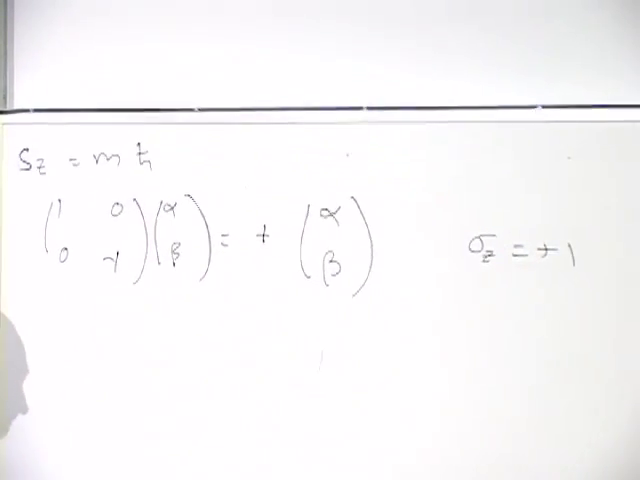
\includegraphics[width=0.74\textwidth]{lecture_08_figure_02.png}
\caption{Ecuación de valores propios de \(+1\) para \(\sigma_z\) al actuar sobre un espinor de dos componentes.}
\lectureframe{00:34:57}
\end{figure}

Para el valor propio \(+1\), la multiplicación fila por fila da
\begin{equation}
\begin{pmatrix}
1\cdot\alpha+0\cdot\beta\\
0\cdot\alpha-\beta
\end{pmatrix}
=
\begin{pmatrix}
\alpha\\
-\beta
\end{pmatrix}
=
\begin{pmatrix}
\alpha\\
\beta
\end{pmatrix}.
\end{equation}
La ecuación superior se cumple automáticamente, mientras que la inferior da \(-\beta=\beta\) y, por tanto, \(\beta=0\). La normalización exige \(|\alpha|=1\); eligiendo la fase global irrelevante de modo que \(\alpha=1\),
\begin{equation}
|+z\rangle=
\begin{pmatrix}
1\\
0
\end{pmatrix}.
\end{equation}

Para el valor propio \(-1\),
\begin{equation}
\begin{pmatrix}
\alpha\\
-\beta
\end{pmatrix}
=
\begin{pmatrix}
-\alpha\\
-\beta
\end{pmatrix}.
\end{equation}
Ahora la ecuación inferior se cumple automáticamente y la superior da \(\alpha=-\alpha\), de modo que \(\alpha=0\). Al elegir \(\beta=1\) se obtiene
\begin{equation}
|-z\rangle=
\begin{pmatrix}
0\\
1
\end{pmatrix}.
\end{equation}

Ahora cambiemos el experimento y midamos \(S_x\). Como
\begin{equation}
\sigma_x
\begin{pmatrix}
\alpha\\
\beta
\end{pmatrix}
=
\begin{pmatrix}
0\cdot\alpha+\beta\\
\alpha+0\cdot\beta
\end{pmatrix}
=
\begin{pmatrix}
\beta\\
\alpha
\end{pmatrix},
\end{equation}
la ecuación para \(+1\) se convierte en
\begin{equation}
\begin{pmatrix}
\beta\\
\alpha
\end{pmatrix}
=
\begin{pmatrix}
\alpha\\
\beta
\end{pmatrix}.
\end{equation}
Las dos ecuaciones para las componentes, \(\beta=\alpha\) y \(\alpha=\beta\), expresan la misma condición. La normalización da
\begin{equation}
2|\alpha|^2=1,
\end{equation}
por lo que una elección conveniente es
\begin{equation}
|+x\rangle
=
\frac{1}{\sqrt2}
\begin{pmatrix}
1\\
1
\end{pmatrix}.
\end{equation}

\begin{figure}[t]
\centering
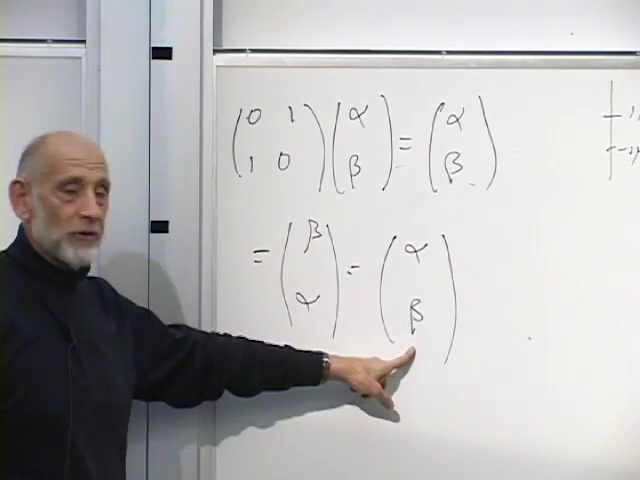
\includegraphics[width=0.74\textwidth]{lecture_08_figure_03.png}
\caption{Para el valor propio \(+1\), \(\sigma_x\) intercambia las dos componentes, por lo que se requiere \(\alpha=\beta\).}
\lectureframe{00:39:42}
\end{figure}

\begin{classroomqa}
\lecturetimestamp{00:40:13}
\audiencequestion{Si se incluyera el factor de un medio, ¿el valor propio sería un medio?}
\lecturerresponse{Sí. La matriz de Pauli \(\sigma_x\) tiene valores propios \(\pm1\), mientras que \(S_x=\sigma_x/2\) tiene valores propios \(\pm\tfrac12\).}
\end{classroomqa}

Para el valor propio \(-1\),
\begin{equation}
\begin{pmatrix}
\beta\\
\alpha
\end{pmatrix}
=
-
\begin{pmatrix}
\alpha\\
\beta
\end{pmatrix},
\end{equation}
por tanto,
\begin{equation}
\beta=-\alpha,
\qquad
\alpha=-\beta.
\end{equation}
De nuevo, estas son la misma ecuación. Tras normalizar,
\begin{equation}
|-x\rangle
=
\frac{1}{\sqrt2}
\begin{pmatrix}
1\\
-1
\end{pmatrix}.
\end{equation}
Así, una superposición equiponderada de espín hacia arriba según \(z\) y hacia abajo según \(z\) está polarizada a lo largo del eje \(x\) positivo, mientras que la misma superposición con un signo relativo menos está polarizada a lo largo del eje \(x\) negativo.

Para la dirección \(y\),
\begin{equation}
\sigma_y
\begin{pmatrix}
\alpha\\
\beta
\end{pmatrix}
=
\begin{pmatrix}
-i\beta\\
i\alpha
\end{pmatrix}.
\end{equation}
Los dos vectores propios normalizados son
\begin{equation}
|+y\rangle
=
\frac{1}{\sqrt2}
\begin{pmatrix}
1\\
i
\end{pmatrix},
\qquad
|-y\rangle
=
\frac{1}{\sqrt2}
\begin{pmatrix}
1\\
-i
\end{pmatrix},
\end{equation}
salvo una fase global. Ambos estados dan probabilidad \(1/2\) de espín hacia arriba respecto de \(z\) y \(1/2\) de espín hacia abajo respecto de \(z\). La fase relativa \(i\), invisible en esas dos probabilidades, distingue la polarización en la dirección \(y\) de la polarización en la dirección \(x\). Las combinaciones lineales también describen el espín polarizado en direcciones arbitrarias; ese cálculo se deja para más adelante.

\begin{classroomqa}
\lecturetimestamp{00:44:22}
\audiencequestion{¿Se ha asignado el signo de la componente \(i\) al valor propio \(\sigma_y\) equivocado?}
\lecturerresponse{Es posible que el signo se haya asignado al valor propio equivocado. Aquí la asignación es incierta; no se está fijando de memoria.}
\end{classroomqa}

La comprobación directa es
\begin{align}
\sigma_y\frac{1}{\sqrt2}
\begin{pmatrix}
1\\
i
\end{pmatrix}
&=
\frac{1}{\sqrt2}
\begin{pmatrix}
-i\,i\\
i
\end{pmatrix}
=
\frac{1}{\sqrt2}
\begin{pmatrix}
1\\
i
\end{pmatrix},\\
\sigma_y\frac{1}{\sqrt2}
\begin{pmatrix}
1\\
-i
\end{pmatrix}
&=
\frac{1}{\sqrt2}
\begin{pmatrix}
(-i)(-i)\\
i
\end{pmatrix}
=
-\frac{1}{\sqrt2}
\begin{pmatrix}
1\\
-i
\end{pmatrix}.
\end{align}
Así, \(+i\) corresponde al valor propio \(+1\), y \(-i\) corresponde al valor propio \(-1\).\footnote{La asignación hecha oralmente sigue sin resolverse tras varias rectificaciones; los signos que se muestran aquí quedan fijados por la multiplicación matricial indicada.} Todo estado de espín un medio, incluidos los polarizados en direcciones arbitrarias, es una combinación lineal de \(|+z\rangle\) y \(|-z\rangle\).

\section{Espín uno y espinores dependientes de la posición}

Para espín \(1\), los valores posibles de \(S_z\) son \(+1,0,-1\). Por tanto, el espacio de estados es tridimensional. El espín \(1\) es entero y corresponde a estadística bosónica. Buscamos tres matrices \(3\times3\) que satisfagan los mismos conmutadores del momento angular.

A continuación se presenta una representación simétrica respecto de las tres direcciones coordenadas.\footnote{El signo de \(S_y\) viene determinado por la matriz que se muestra cerca de \(00{:}48{:}50\) y también queda fijado por \([S_x,S_y]=iS_z\). Cambiar ese signo invertiría el conmutador requerido.}
\begin{equation}
\begin{aligned}
S_x
&=
i
\begin{pmatrix}
0&0&0\\
0&0&1\\
0&-1&0
\end{pmatrix},
&
S_y
&=
i
\begin{pmatrix}
0&0&1\\
0&0&0\\
-1&0&0
\end{pmatrix},\\
S_z
&=
i
\begin{pmatrix}
0&1&0\\
-1&0&0\\
0&0&0
\end{pmatrix}.
\end{aligned}
\end{equation}
Cada matriz es \(i\) por una matriz real antisimétrica. Cada una contiene un \(1\), un \(-1\) y una fila y una columna nulas asociadas a su propia coordenada: la primera para \(S_x\), la segunda para \(S_y\) y la tercera para \(S_z\). Esto proporciona una regla mnemotécnica útil. En esta representación, \(S_z\) no es diagonal.

Sea
\begin{equation}
v=
\begin{pmatrix}
\alpha\\
\beta\\
\gamma
\end{pmatrix}.
\end{equation}
Entonces
\begin{equation}
S_zv
=
\begin{pmatrix}
i\beta\\
-i\alpha\\
0
\end{pmatrix}.
\end{equation}
Para el valor propio \(+1\),
\begin{equation}
i\beta=\alpha,
\qquad
-i\alpha=\beta,
\qquad
0=\gamma.
\end{equation}
Así, \(\beta=-i\alpha\) y \(\gamma=0\). La normalización da \(2|\alpha|^2=1\), por lo que
\begin{equation}
|m=+1\rangle
=
\frac{1}{\sqrt2}
\begin{pmatrix}
1\\
-i\\
0
\end{pmatrix}.
\end{equation}
Para el valor propio \(-1\),
\begin{equation}
i\beta=-\alpha,
\qquad
-i\alpha=-\beta,
\qquad
0=-\gamma,
\end{equation}
de donde \(\beta=i\alpha\), \(\gamma=0\) y
\begin{equation}
|m=-1\rangle
=
\frac{1}{\sqrt2}
\begin{pmatrix}
1\\
i\\
0
\end{pmatrix}.
\end{equation}
Por último, la ecuación para el valor propio cero da \(\alpha=\beta=0\), y deja \(\gamma\) arbitrario. Su solución normalizada es
\begin{equation}
|m=0\rangle
=
\begin{pmatrix}
0\\
0\\
1
\end{pmatrix}.
\end{equation}
No hay más valores propios: estos tres vectores propios agotan el espacio tridimensional. Los factores \(1/\sqrt2\) no son meramente decorativos. Más adelante, cuando se aplique el álgebra al isospín, los mismos coeficientes intervendrán en predicciones experimentales cuantitativas.

\begin{classroomqa}
\lecturetimestamp{00:54:10}
\audiencequestion{¿Cómo se deben interpretar las componentes complejas de estos vectores propios de espín uno?}
\lecturerresponse{Para \(m=+1\), las componentes son \(1/\sqrt2,-i/\sqrt2,0\); para \(m=-1\), son \(1/\sqrt2,i/\sqrt2,0\); y para \(m=0\), son \(0,0,1\).}
\end{classroomqa}

Otras ternas de matrices satisfacen la misma álgebra y son físicamente equivalentes. La representación simétrica anterior resulta útil porque trata por igual las tres direcciones, y se volverá a utilizar.

\subsection{Restitución de la posición}

Ahora restituyamos el movimiento de la partícula. El espín conmuta con la posición y con el momento, así que es posible especificar cualquiera de ellos junto con una componente del espín. La posición y el momento no conmutan, y las distintas componentes del espín tampoco conmutan entre sí.

Una partícula de espín un medio en movimiento se describe mediante un espinor dependiente de la posición,
\begin{equation}
\psi(x)=
\begin{pmatrix}
\psi_\uparrow(x)\\
\psi_\downarrow(x)
\end{pmatrix}.
\end{equation}
Las cantidades
\begin{equation}
\rho_{\uparrow_z}(x)=|\psi_\uparrow(x)|^2,
\qquad
\rho_{\downarrow_z}(x)=|\psi_\downarrow(x)|^2
\end{equation}
son densidades de probabilidad conjuntas de posición y espín. Su suma,
\begin{equation}
\rho(x)=\psi^\dagger(x)\psi(x)
=|\psi_\uparrow(x)|^2+|\psi_\downarrow(x)|^2,
\end{equation}
es la densidad de posición. Si se sabe que la partícula se detectó en \(x\), las probabilidades condicionadas son
\begin{equation}
P(\uparrow_z\mid x)
=
\frac{|\psi_\uparrow(x)|^2}{\psi^\dagger(x)\psi(x)},
\qquad
P(\downarrow_z\mid x)
=
\frac{|\psi_\downarrow(x)|^2}{\psi^\dagger(x)\psi(x)},
\end{equation}
siempre que \(\rho(x)\neq0\). Así, un electrón se representa mediante una función de onda espacial de dos componentes, cuyas amplitudes locales de espín pueden variar de un lugar a otro.

Para una partícula de espín uno en movimiento, escribamos
\begin{equation}
\phi(x)=
\begin{pmatrix}
\phi_1(x)\\
\phi_2(x)\\
\phi_3(x)
\end{pmatrix}.
\end{equation}
En cada punto del espacio, las tres componentes forman un vector en el mismo espacio de espín empleado antes. Las partículas de espín uno tienen espín entero y son bosones.

\begin{classroomqa}
\lecturetimestamp{01:00:10}
\audiencequestion{¿Es \(\phi_1(x)\) la probabilidad del resultado de espín uno \(m=+1\)?}
\lecturerresponse{No. Es una amplitud en la base elegida de tres componentes. Para obtener un resultado definido de espín, se forma el bra del vector propio normalizado correspondiente, se proyecta el campo sobre él y se toma el módulo al cuadrado.}
\end{classroomqa}

\begin{figure}[t]
\centering
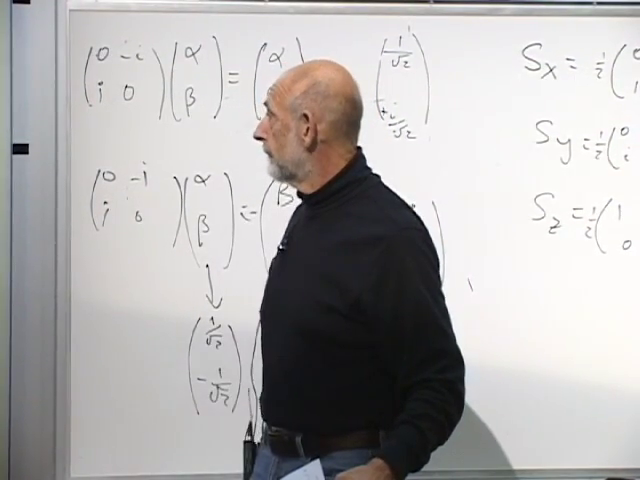
\includegraphics[width=0.82\textwidth]{lecture_08_figure_04.png}
\caption{Vectores propios normalizados de \(\sigma_y\) junto a las tres matrices de espín uno mitad.}
\lectureframe{01:00:12}
\end{figure}

Por ejemplo,
\begin{equation}
\begin{aligned}
|m=+1\rangle
&=
\frac{1}{\sqrt2}
\begin{pmatrix}
1\\
-i\\
0
\end{pmatrix}
\\
\Longrightarrow\quad\langle m=+1|
&=
\frac{1}{\sqrt2}
\begin{pmatrix}
1&i&0
\end{pmatrix}.
\end{aligned}
\end{equation}
Por tanto, la amplitud de proyección es
\begin{align}
\langle m=+1|\phi(x)\rangle
&=
\frac{1}{\sqrt2}
\begin{pmatrix}
1&i&0
\end{pmatrix}
\begin{pmatrix}
\phi_1(x)\\
\phi_2(x)\\
\phi_3(x)
\end{pmatrix}\\
&=
\frac{\phi_1(x)+i\phi_2(x)}{\sqrt2}.
\end{align}
Aplicando la misma regla a los tres vectores propios se obtienen las densidades resueltas según el espín.\footnote{Estas fórmulas completan el álgebra de proyección tras la corrección explícita de que \(\phi_1\) y \(\phi_2\) no tienen por qué ser reales. Tratarlas como reales borraría incorrectamente la interferencia que distingue las densidades \(m=+1\) y \(m=-1\).}
\begin{align}
\rho_{+1}(x)
&=
\frac12\left|\phi_1(x)+i\phi_2(x)\right|^2,\\
\rho_{-1}(x)
&=
\frac12\left|\phi_1(x)-i\phi_2(x)\right|^2,\\
\rho_0(x)
&=
|\phi_3(x)|^2.
\end{align}
Satisfacen
\begin{equation}
\begin{aligned}
\rho_{+1}(x)+\rho_{-1}(x)+\rho_0(x)
&=
|\phi_1(x)|^2+|\phi_2(x)|^2
\\
&\quad{}+|\phi_3(x)|^2
\\
&=
\phi^\dagger(x)\phi(x).
\end{aligned}
\end{equation}
Si se condiciona a que la partícula se detectó en \(x\), entonces
\begin{equation}
P(m\mid x)
=
\frac{\rho_m(x)}{\phi^\dagger(x)\phi(x)},
\end{equation}
siempre que \(\phi^\dagger(x)\phi(x)\neq0\). La regla general de medición es siempre la misma: se forma el bra del vector propio normalizado deseado, se proyecta sobre él el estado real y se toma el módulo al cuadrado. La densidad resultante conserva su dependencia de la posición.

Las matrices de espín más alto son más complicadas, pero el principio no cambia.

\begin{classroomqa}
\lecturetimestamp{01:07:31}
\audiencequestion{¿Cuál es la dimensión del espacio de estados para espín tres mitades?}
\lecturerresponse{Tiene cuatro estados, con \(m=\tfrac32,\tfrac12,-\tfrac12,-\tfrac32\). El espín dos tiene cinco estados.}
\end{classroomqa}

\begin{classroomqa}
\lecturetimestamp{01:07:55}
\audiencequestion{¿Por qué se ha hablado de \(x,y,z\) sin mencionar ninguna dirección temporal? ¿Es no relativista este tratamiento?}
\lecturerresponse{Hasta ahora es no relativista. El espín, al igual que la masa, se caracteriza más fácilmente en el sistema de reposo de la partícula; su descripción en otro sistema inercial se obtiene mediante la transformación de Lorentz apropiada. Ese paso relativista se deja para más adelante.}
\end{classroomqa}

La ecuación de Dirac proporciona el marco relativista y explica por qué su función de onda de cuatro componentes contiene un doblete de espín.

\section{Matrices de Dirac y espinor de cuatro componentes}

La función de onda de Dirac de cuatro componentes satisface
\begin{equation}
i\frac{\partial\Psi}{\partial t}
=
-i\alpha_i\frac{\partial\Psi}{\partial x_i}
+m\beta\Psi,
\qquad i=1,2,3,
\end{equation}
donde se suma sobre un índice espacial repetido. Por tanto, el término con derivadas significa
\begin{equation}
\alpha_1\frac{\partial\Psi}{\partial x}
+\alpha_2\frac{\partial\Psi}{\partial y}
+\alpha_3\frac{\partial\Psi}{\partial z}.
\end{equation}
Para una onda plana, esto se convierte en la ecuación algebraica
\begin{equation}
\omega\Psi=(\alpha_i k_i+m\beta)\Psi.
\end{equation}

\begin{classroomqa}
\lecturetimestamp{01:11:32}
\audiencequestion{¿Las dos apariciones de \(m\) denotan lo mismo?}
\lecturerresponse{No. Una se estaba usando como índice espacial y la otra representa la masa de la partícula. Cambiemos el índice espacial por \(i\); cuando \(i\) aparece dos veces, se suma desde \(1\) hasta \(3\).}
\end{classroomqa}

Al elevar al cuadrado el operador de frecuencia se debe recuperar la relación relativista
\begin{equation}
\omega^2=\mathbf{k}^2+m^2.
\end{equation}
Por tanto, los términos de los cuadrados exigen, para cada \(i\),
\begin{equation}
\alpha_i^2=I_4,
\qquad
\beta^2=I_4.
\end{equation}

\begin{classroomqa}
\lecturetimestamp{01:13:01}
\audiencequestion{¿Es \(\beta\) distinto para cada una de las cuatro componentes de \(\Psi\)?}
\lecturerresponse{No. Hay una única matriz \(\beta\), que actúa sobre el espinor completo de cuatro componentes y satisface \(\beta^2=I_4\).}
\end{classroomqa}

Los términos mixtos deben anularse. Para direcciones espaciales distintas, y también entre cada \(\alpha_i\) y \(\beta\), se obtiene
\begin{equation}
\alpha_i\alpha_j+\alpha_j\alpha_i=0
\quad (i\neq j),
\qquad
\alpha_i\beta+\beta\alpha_i=0.
\end{equation}
De manera equivalente,
\begin{equation}
\{\alpha_i,\alpha_j\}=2\delta_{ij}I_4,
\quad
\{\alpha_i,\beta\}=0,
\quad
\{\beta,\beta\}=2I_4.
\end{equation}
Cada matriz anticonmuta con todas las matrices distintas, mientras que su anticonmutador consigo misma es el doble de la identidad.

Sin \(\beta\), las tres matrices de Pauli ya proporcionarían tres matrices \(2\times2\) cuyo cuadrado es la identidad y que anticonmutan por pares. El término de masa exige una cuarta matriz con esas propiedades. No existe una cuarta matriz \(2\times2\) con las propiedades requeridas, y las matrices \(3\times3\) tampoco resuelven el álgebra. Por tanto, la representación más pequeña es \(4\times4\).

Una matriz \(4\times4\) puede dividirse en cuatro bloques \(2\times2\). En una representación conveniente,
\begin{equation}
\alpha_i=
\begin{pmatrix}
\sigma_i&0\\
0&-\sigma_i
\end{pmatrix},
\qquad i=1,2,3.
\end{equation}

\begin{figure}[t]
\centering
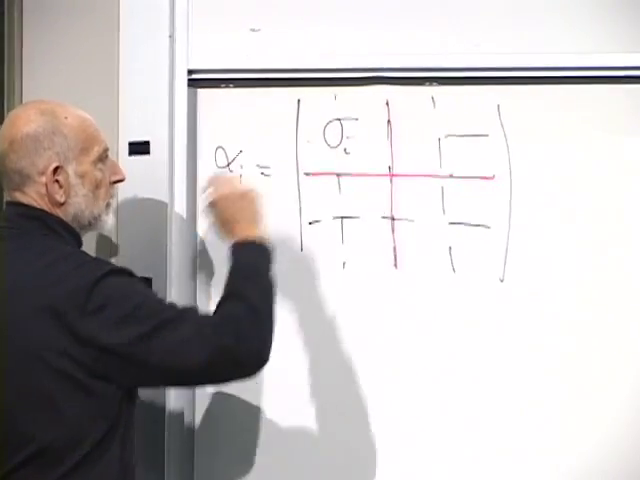
\includegraphics[width=0.68\textwidth]{lecture_08_figure_05.png}
\caption{La matriz de Dirac \(\alpha_i\) escrita en bloques de \(2\times2\), con \(\sigma_i\) y \(-\sigma_i\) en la diagonal.}
\lectureframe{01:17:23}
\end{figure}

\begin{classroomqa}
\lecturetimestamp{01:17:41}
\audiencequestion{¿Estaban dispuestos de otra manera los bloques \(\sigma_i\) en la representación anterior?}
\lecturerresponse{Sí. En otra representación se situaban fuera de la diagonal. Ambas disposiciones son equivalentes y están relacionadas mediante una transformación de semejanza.}
\end{classroomqa}

En la representación actual, la matriz restante es
\begin{equation}
\beta=
\begin{pmatrix}
0&I_2\\
I_2&0
\end{pmatrix},
\qquad
I_2=
\begin{pmatrix}
1&0\\
0&1
\end{pmatrix}.
\end{equation}
La multiplicación por bloques reduce las comprobaciones del álgebra de \(4\times4\) a multiplicaciones ordinarias de matrices \(2\times2\).

\begin{classroomqa}
\lecturetimestamp{01:19:17}
\audiencequestion{¿La representación anterior usaba un signo distinto o una forma diagonal para \(\beta\)?}
\lecturerresponse{Usaba una base distinta, pero físicamente equivalente. Un cambio de base mezcla las cuatro componentes de \(\Psi\) y modifica la forma de las matrices sin alterar la física.}
\end{classroomqa}

Las cuatro componentes de \(\Psi\) no son las cuatro coordenadas del espacio-tiempo. Son coordenadas en el espacio vectorial de menor dimensión sobre el que puede actuar esta álgebra de anticonmutación. Hay dos estructuras distintas de dos componentes: la división en bloques \(2\times2\) y la estructura de Pauli de dos componentes dentro de cada bloque. Anticipando la interpretación que se establecerá más adelante, las cuatro posibilidades pueden organizarse así:
\begin{equation}
\begin{array}{c|cc}
& S_z=+\tfrac12 & S_z=-\tfrac12\\ \hline
\omega>0 & (\omega>0,+\tfrac12) & (\omega>0,-\tfrac12)\\
\omega<0 & (\omega<0,+\tfrac12) & (\omega<0,-\tfrac12)
\end{array}.
\end{equation}
La fila inferior consta de estados electrónicos de frecuencia negativa. No es una fila de positrones; el positrón se interpretará como un hueco en el conjunto lleno de esos estados.

\section{Duplicación de la energía en reposo y el positrón}

La estructura energética doble se ve con mayor facilidad cuando el momento es cero. Cuando \(\mathbf{k}=0\), el estado de onda plana es espacialmente constante y desaparece el término de derivadas espaciales. La ecuación en el sistema de reposo\footnote{En el instante \(01{:}23{:}38\) se conserva transitoriamente un factor adicional de \(i\) en el término de masa; la corrección oral de \(01{:}24{:}05\) lo elimina.} es
\begin{equation}
i\frac{\partial\Psi}{\partial t}=m\beta\Psi.
\end{equation}

\begin{figure}[t]
\centering
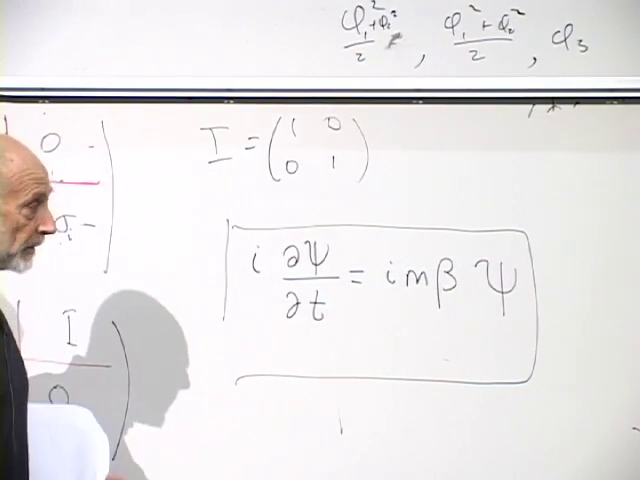
\includegraphics[width=0.76\textwidth]{lecture_08_figure_06.png}
\caption{Con momento nulo, las derivadas espaciales se anulan y queda la ecuación corregida en el sistema de reposo \(i\partial_t\Psi=m\beta\Psi\).}
\lectureframe{01:23:38}
\end{figure}

Dividamos la columna de cuatro componentes en un objeto de dos componentes superior y otro inferior:
\begin{equation}
\Psi=
\begin{pmatrix}
\psi_+\\
\psi_-
\end{pmatrix}.
\end{equation}

\begin{classroomqa}
\lecturetimestamp{01:24:47}
\audiencequestion{¿Las etiquetas \(\psi_+\) y \(\psi_-\) ya significan energía positiva y negativa?}
\lecturerresponse{No. En esta etapa solo son nombres para los bloques superior e inferior de dos componentes. Aún no se han hallado sus combinaciones de energía.}
\end{classroomqa}

\begin{classroomqa}
\lecturetimestamp{01:25:10}
\audiencequestion{¿Qué representa la columna de cuatro componentes dividida?}
\lecturerresponse{Es el mismo espinor de Dirac de cuatro componentes, organizado para ajustarse a la forma en bloques de las matrices. Cada mitad es un objeto de dos componentes y, juntas, forman la columna original de cuatro componentes.}
\end{classroomqa}

La matriz \(\beta\) intercambia los dos bloques:
\begin{equation}
\beta
\begin{pmatrix}
\psi_+\\
\psi_-
\end{pmatrix}
=
\begin{pmatrix}
\psi_-\\
\psi_+
\end{pmatrix}.
\end{equation}
Por tanto, la ecuación en el sistema de reposo queda
\begin{equation}
i\frac{\partial\psi_+}{\partial t}=m\psi_-,
\qquad
i\frac{\partial\psi_-}{\partial t}=m\psi_+.
\end{equation}

Hay dos opciones naturales. Tomar otra derivada temporal desacoplaría el sistema, pero sumar y restar las dos ecuaciones las diagonaliza de inmediato. En efecto,
\begin{align}
i\frac{\partial}{\partial t}(\psi_++\psi_-)
&=m(\psi_++\psi_-),\\
i\frac{\partial}{\partial t}(\psi_+-\psi_-)
&=-m(\psi_+-\psi_-).
\end{align}
Definiendo
\begin{equation}
\chi_+=\psi_++\psi_-,
\qquad
\chi_-=\psi_+-\psi_-,
\end{equation}
se obtienen dos ecuaciones independientes,
\begin{equation}
i\partial_t\chi_+=m\chi_+,
\qquad
i\partial_t\chi_-=-m\chi_-.
\end{equation}
Para una dependencia temporal de frecuencia definida \(e^{-i\omega t}\), la suma tiene
\begin{equation}
\omega=+m,
\end{equation}
mientras que la diferencia tiene
\begin{equation}
\omega=-m.
\end{equation}
Este es exactamente el desdoblamiento en energías positiva y negativa que apareció en el ejemplo unidimensional anterior: la ecuación relativista vuelve a tener soluciones electrónicas de energía positiva y negativa. Así, el desdoblamiento en bloques se separa en ramas de energía positiva y negativa. Los estados puros en el sistema de reposo pueden escribirse como
\begin{equation}
\Psi_{\omega=+m}=
\begin{pmatrix}
\xi\\
\xi
\end{pmatrix},
\qquad
\Psi_{\omega=-m}=
\begin{pmatrix}
\xi\\
-\xi
\end{pmatrix},
\end{equation}
donde \(\xi\) sigue siendo un objeto arbitrario de dos componentes.

La suma y la diferencia han eliminado una estructura de dos posibilidades, pero aún quedan las dos componentes de \(\xi\). Las matrices de Pauli actúan sobre este par residual. Este es el par asociado al espín, sujeto a la comprobación de rotación y de las leyes de conservación que se analiza más adelante.

\begin{classroomqa}
\lecturetimestamp{01:32:23}
\audiencequestion{¿Se puede considerar el espín como la estructura externa de dos posibilidades y el signo de la energía como la interna?}
\lecturerresponse{Sí. Los dos ordenamientos de factores son equivalentes. Se puede intercambiar qué índice se escribe primero; el cambio consiste únicamente en reordenar las cuatro componentes.}
\end{classroomqa}

La rama de frecuencia negativa conduce a la interpretación del mar de Dirac. A una frecuencia negativa se le asigna energía electrónica negativa. Al llenar todos los estados electrónicos de energía negativa, la energía disminuye tanto como permite el principio de exclusión, pues cada estado fermiónico completo puede estar ocupado por un solo electrón. Al mar de energía negativa completamente lleno se le llama entonces vacío.

Se promueve un electrón de este mar lleno a un estado de energía positiva. El resultado contiene un electrón de energía positiva y un estado de energía negativa desocupado. Al quitar una energía negativa, la energía aumenta, de modo que el hueco tiene energía de excitación positiva; como falta un electrón, también tiene la carga eléctrica opuesta. El hueco es un positrón.

\begin{classroomqa}
\lecturetimestamp{01:32:57}
\audiencequestion{¿Se puede explicar una vez más la interpretación del positrón?}
\lecturerresponse{La suma de los dos bloques tiene frecuencia positiva y la diferencia tiene frecuencia negativa. Las soluciones de frecuencia negativa son estados electrónicos de energía negativa, y el vacío se obtiene llenándolos todos. Al promover un electrón lleno a energía positiva, quedan tanto un electrón de energía positiva como un hueco. Ese hueco de energía positiva y carga opuesta es el positrón.}
\end{classroomqa}

Por tanto, el álgebra ha producido a la vez dos consecuencias: ramas de energía positiva y negativa, que dan lugar a la estructura partícula--antipartícula, y una estructura residual de dos componentes asociada al espín uno medio. Lo sorprendente es que ambas surgieran de las matrices más pequeñas capaces de satisfacer las relaciones relativistas de anticonmutación. El espín había aparecido hacía poco como propiedad empírica cuando esta construcción matemática produjo partículas con espín, junto con una rama de antipartículas; en aquel contexto histórico, el resultado fue extraordinario.

\begin{classroomqa}
\lecturetimestamp{01:35:14}
\audiencequestion{¿Son positrones los propios electrones de energía negativa?}
\lecturerresponse{No. Los estados electrónicos de energía negativa están llenos en el vacío. Un positrón es la ausencia de un electrón de ese conjunto lleno: un hueco, no un electrón de energía negativa.}
\end{classroomqa}

Un hueco puede participar en transiciones. Un positrón tiene energía positiva porque es la ausencia de un electrón de energía negativa. Si un electrón de energía positiva ocupa el hueco, el electrón y el positrón se aniquilan, pero su energía debe ser transportada, normalmente por fotones. En el lenguaje del mar, un electrón ha ocupado un estado de energía negativa desocupado. La misma liberación de energía puede imaginarse como un electrón excitado de un átomo que desciende a un nivel inferior: la transición descendente emite fotones.

\begin{classroomqa}
\lecturetimestamp{01:36:39}
\audiencequestion{¿Por qué los electrones de energía negativa más alta no caen en el hueco?}
\lecturerresponse{Esa pregunta mezcla dos casos. Que un electrón de energía positiva ocupe el hueco es la aniquilación electrón--positrón, en la que los fotones se llevan la energía. La transición de un electrón del mar de energía negativa es un proceso distinto, que se aborda más adelante.}
\end{classroomqa}

El cálculo con momento nulo por sí solo ha establecido una degeneración doble una vez separado el signo de la energía. La degeneración de dos estados no demuestra, por sí misma, que esos estados tengan momento angular.

\begin{classroomqa}
\lecturetimestamp{01:37:44}
\audiencequestion{¿Cómo demuestra el cálculo con momento nulo que el par de estados restante es espín?}
\lecturerresponse{Se puede llamar arriba y abajo al par, y las matrices de Pauli aparecen en la ecuación completa, pero eso por sí solo aún no lo demuestra. Hay que mostrar cómo se transforma el par bajo rotaciones espaciales, o bien que al asignarle espín se conserva el momento angular total en las interacciones y colisiones. Esa demostración se deja para más adelante.}
\end{classroomqa}

Para un estado de energía positiva en reposo, los bloques superior e inferior son iguales,
\begin{equation}
\Psi_{\omega=+m}=
\begin{pmatrix}
\xi\\
\xi
\end{pmatrix}.
\end{equation}
Demostrar que \(\xi\) es un doblete de momento angular requiere el argumento basado en las rotaciones o en la conservación que se acaba de describir; no se deduce simplemente de contar dos componentes.

\begin{classroomqa}
\lecturetimestamp{01:40:46}
\audiencequestion{¿Puede aniquilarse con el positrón otro electrón aunque tenga una energía distinta?}
\lecturerresponse{Sí. Los electrones no conservan una identidad individual. Cualquiera de los electrones disponibles puede ocupar el hueco, y las diferencias de energía y momento iniciales se reflejan en el número y las energías de los fotones emitidos.}
\end{classroomqa}

La imagen del hueco también explica una transición que ocurre por completo dentro del mar de energía negativa. Supongamos que un estado ocupado de energía negativa pasa al hueco. El hueco original queda ocupado, pero el estado del que procedía ese electrón queda ahora vacío. El hueco se ha desplazado. De forma equivalente, el positrón ha cambiado de energía y ha emitido radiación.

\begin{classroomqa}
\lecturetimestamp{01:42:12}
\audiencequestion{¿Por qué los niveles de energía negativa vecinos no pueden caer sucesivamente en el hueco?}
\lecturerresponse{Pueden desplazar el hueco de un nivel a otro. Un electrón que cae en el hueco anterior deja un nuevo hueco en la energía que ocupaba, de modo que el positrón inicial pasa a tener otra energía. La diferencia de energía la transportan los fotones.}
\end{classroomqa}

\begin{classroomqa}
\lecturetimestamp{01:44:39}
\audiencequestion{¿Por qué esto no produce una cascada radiativa descendente sin fin?}
\lecturerresponse{Porque la energía y el momento deben conservarse simultáneamente. Esas dos leyes de conservación no permiten que el proceso ocurra sin restricciones. El mismo problema aparece con un electrón libre ordinario: no puede seguir reduciendo su energía mediante la emisión de fotones en el espacio vacío.}
\end{classroomqa}
